
\section{Introduction}
\label{sec:introduction}
%%% General intro
\IEEEPARstart{T}{he} constant research and the rapid evolution of artificial neural network (ANN) architectures are driving the transition to smarter and more powerful AI applications, where CNN-based models represent the essential building blocks of deep learning algorithms in computer vision tasks \cite{hassaballah2020deep}. Applications such as smart surveillance, medical imaging, natural language processing, robotics, and autonomous navigation have been powered by CNN-based models in industry and academia \cite{dhillon2020convolutional}. Nonetheless, dedicated hardware is often a requirement to accelerate execution due to the high computational demands of CNNs. In terms of pure computational throughput, graphics processing units (GPUs) offer the best performance\cite{nurvitadhi2017can}. In terms of power consumption, FPGA solutions are well known to be more energy efficient (vs GPUs). As a result, numerous FPGA accelerators have been proposed, targeting both high performance computing (HPC) for data-centers and embedded systems applications \cite{abdelouahab2018accelerating}. However, most commercial deep learning processing units (DPUs) are not designed for low-power, resource-limited embedded FPGAs.

In this paper, we present a hardware/software co-design framework to accelerate tensor operators for TF Lite Micro on resource-constrained and low-power embedded FPGAs. Based on their high computational cost, in this paper, we accelerate Conv2D and DepthwiseConv2D operators. The proposed architecture supports TF Lite quantized models with int8 and standard float32. To enhance resource utilization and energy consumption, the tensor operators are designed as separate hardware engines, where they are optionally instantiated in the FPGA fabric. To accelerate floating-point computation, we propose a decomposed floating-point calculation for the vector dot-product. To enhance on-chip memory usage and for quality reconfigurability, the proposed design employs hybrid custom floating-point formats, where filter and bias tensors are quantized and stored with a reduced format on the hardware accelerator. The hardware design is implemented with high-level synthesis (HLS).

\begin{figure}[t!]
	\centering
	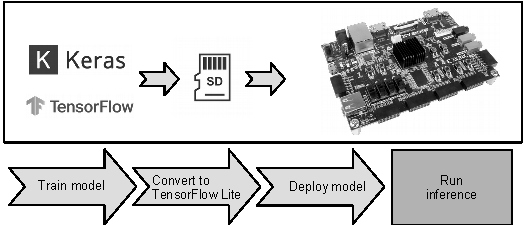
\includegraphics[width=0.5\textwidth]{../figures/workflow.pdf}
	\caption{Deployment workflow.}
	\label{fig:workflow}
\end{figure}

To operate the proposed accelerator framework, we train a CNN model on TensorFlow or Keras, then this is converted into a TensorFlow Lite model with either float32 or int8 quantization, then the model is stored in a micro SD card along with the software and the FPGA configuration bitstream for deployment. See \Fig{fig:workflow}.

To demonstrate the potential of the proposed framework, we address a design exploration with two custom-built CNN architectures for CIFAR-10 image classification. We demonstrate the performance of the Conv2D and DepthwiseConv2D operator engines with fixed-pint quantization, floating-point with Xilinx LogiCORE IP, decomposed floating-point with single precision, half-precision, brain floating-point, TensorFloat, and custom reduced formats for approximate processing, including logarithmic computation. We present a detailed runtime computation schedule and an exhaustive accuracy performance using custom reduced floating-point formats.

A single accelerator running at 150 MHz on a Xilinx Zynq-7020 achieves 45X runtime acceleration on Conv2D tensor operation compared with ARM Cortex-A9 at 666MHz, and 5X compared with the equivalent standard floating-point implementation in HLS with Xilinx LogiCORE IP. This accelerator yields a peak performance of 1.6 TFLOPS/watt and 152 MFLOP/s. The entire hardware design and the implemented TF Lite software extensions are available as an open-source project.